% Chapter Template

\chapter{实验设计} % Main chapter title

\label{Chapter3} % Change X to a consecutive number; for referencing this chapter elsewhere, use \ref{ChapterX}

%----------------------------------------------------------------------------------------
%	SECTION 1
%----------------------------------------------------------------------------------------

\section{CPU流水结构}


%-----------------------------------
%	SUBSECTION 1
%-----------------------------------
\subsection{整体设计}


我们设计并实现了五级流水结构的CPU,对每条指令的处理分为IF、ID、EXE、MEM、WB五个阶段。采用25M时钟,每个时钟周期流水线的每一个阶段完成一条指令的一部分,不同阶段并行完成不同指令的不同部分。同时每两个阶段之间均有一个段间锁存器,用与接收上一阶段的信号并在下一个时钟上升沿到来时传递到下一阶段。

流水线五个阶段的功能与所占用的资源如下:

IF:根据输入的PC值从内存中取出指令。在执行写入命令时,还需要根据PC值向内存中写入用户指令。占用资源:IM、PC、总线

ID:根据IF阶段读取的指令进行译码,从寄存器堆中读出所需寄存器的值。占用资源:寄存器组

EXE:根据ID阶段生成的控制信号、操作数和操作符进行计算,将结果传递到下一阶段。占用资源:ALU

MEM:根据ID阶段生成的控制信号执行写入内存和读取内存的操作,在实现时还需考虑串口的读写与VGA/Keyboard的读写访问。占用资源:DM、总线

WB:根据控制信号执行写回寄存器的操作。占用资源:寄存器组

%-----------------------------------
%	SUBSECTION 2
%-----------------------------------

\subsection{数据通路}

我们设计的数据通路见Figure 3.1.
\begin{figure}[H]
  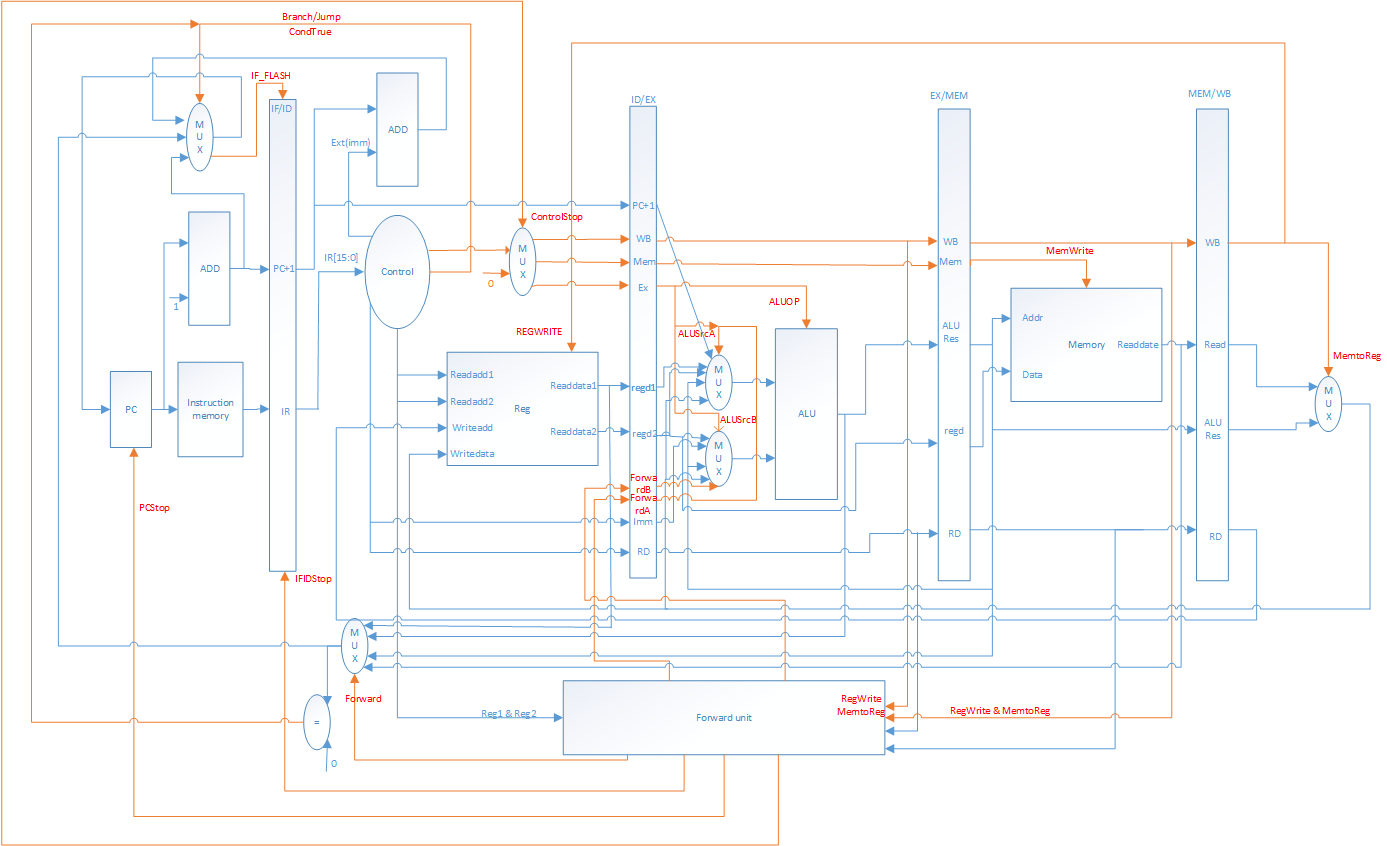
\includegraphics[width=\linewidth]{Figures/datapath.png}
  \caption{数据通路.}
\end{figure}

在数据通路的设计上,我们基本遵循经典的五级流水线结构,但是在其基础之上有了一些变化和改进。

我们将处理数据冲突的模块全部放在了Forward Unit中。既可以将在EXE、MEM的计算结果流回到下一条指令的EXE阶段,同时也可以对访存操作的数据冲突进行插气泡处理。Forward Unit模块还可以处理跳转指令的数据冲突,这样整体结构更加简洁。

我们新增PC模块,同于计算下一周期取指的PC值,根据跳转信号进行计算,可以解决控制冲突。具体实现见冲突处理部分。

%-----------------------------------
%	SUBSECTION 3
%-----------------------------------

\subsection{控制信号}
在ID阶段译码的过程中,会产生很多控制信号,针对我们所需实现的30条指令的指令集,我们设计的控制信号为:

ALUOP:ALU运算器的操作符,包括的类型有 ADD(加法)、SUB(减法)、ASSIGNA(赋操作数A的值)、ASSIGNB(赋操作数B的值)、AND(与)、OR(或)、SLL(逻辑左移)、SRA(算数右移)、EQUAL(判断相等)、LESS(判断小于)、EMPTY(无操作)。

SRCREGA:读取第一个寄存器值的控制使能。1表示IR[10:8],0表示特殊寄存器。

SRCREGB:读取第二个寄存器值的控制使能。1表示IR[10:8],0表示IR[7:5]。

REGDST:写回寄存器编号的控制使能。00表示特殊寄存器,01表示IR[10:8],10表示IR[7:5],11表示IR[4:2]。

ALUSRCA:ALU运算器第一个操作数的选择信号。00表示Reg[IR[10:8]],01表示Reg[IR[7:5]],10表示EPC。

ALUSRCB:ALU运算器第二个操作数的选择信号。1表示reg[IR[7:5]],0表示extend(imm)。

EXTOP:立即数扩展方式。0表示符号扩展,1表示零扩展。

MEMTOREG:读取内存并写回寄存器使能。

REGWRITE:写回寄存器使能。

MEMWRITE:内存写使能。

BRANCH:B指令跳转信号。00表示无B型跳转,10表示无条件跳转,01表示不等条件跳转,11表示相等条件跳转。

JUMP:J指令跳转使能。

对于每条指令的控制信号,见表3.1—3.5,其中的‘x’表示没有使用。

\begin{table}[H]
\begin{center}
\renewcommand{\arraystretch}{1.3}
\small
\caption{Control Signals}
\label{tab:treatments}
\begin{tabular}{|>{\centering}p{2.1cm}|*{6}{p{1.4cm}<{\centering}}|}
\hline
& ADDIU & ADDIU3 & ADDSP & ADDU & AND & B \\
\hline
ALUOP & ADD	& ADD & ADD & ADD & AND & EMPTY\\	
\hline
SRCREGA & 1 & 1 & 0 & 1 & 1 & x\\
\hline
SRCREGB & x & x & x & 0 & 0 & x\\
\hline
REGDST & 01 & 10 & 00 & 11 & 01 & x\\
\hline
ALUSRCA & 00 & 00 & 00 & 00 & 00 & x\\
\hline
ALUSRCB & 0 & 0 & 0 & 1 & 1 & x\\
\hline
EXTOP & 0 & 0 & 0 & x & x & 0\\
\hline
MEMTOREG & 0 & 0 & 0 & 0 & 0 & 0\\
\hline
REGWRITE & 1 & 1 & 1 & 1 & 1 & 0\\
\hline
MEMWRITE & 0 & 0 & 0 & 0 & 0 & 0\\
\hline
BRANCH & 00 & 00 & 00 & 00 & 00 & 10\\
\hline
JUMP & 0 & 0 & 0 & 0 & 0 & 0\\
\hline
\end{tabular}
\end{center}
\end{table}


\begin{table}[H]
\begin{center}
\renewcommand{\arraystretch}{1.3}
\small
\caption{Control Signals}
\label{tab:treatments}
\begin{tabular}{|>{\centering}p{2.1cm}|*{6}{p{1.4cm}<{\centering}}|}
\hline
& BEQZ & BNEZ & BTEQZ & CMP & CMPI & JALR \\
\hline
ALUOP & EMPTY & EMPTY & EMPTY & EQUAL & EQUAL & ASSIGNA\\	
\hline
SRCREGA & 1 & 1 & 0 & 1 & 1 & 1\\
\hline
SRCREGB & x & x & x & 0 & x & x\\
\hline
REGDST & x & x & x & 00 & 00 & 00\\
\hline
ALUSRCA & x & x & x & 00 & 00 & 10\\
\hline
ALUSRCB & x & x & x & 1 & 0 & x\\
\hline
EXTOP & 0 & 0 & 0 & x & 0 & x\\
\hline
MEMTOREG & 0 & 0 & 0 & 0 & 0 & 0\\
\hline
REGWRITE & 0 & 0 & 0 & 1 & 1 & 1\\
\hline
MEMWRITE & 0 & 0 & 0 & 0 & 0 & 0\\
\hline
BRANCH & 11 & 01 & 11 & 00 & 00 & 00\\
\hline
JUMP & 0 & 0 & 0 & 0 & 0 & 1\\
\hline
\end{tabular}
\end{center}
\end{table}


\begin{table}[H]
\begin{center}
\renewcommand{\arraystretch}{1.3}
\small
\caption{Control Signals}
\label{tab:treatments}
\begin{tabular}{|>{\centering}p{2.1cm}|*{6}{p{1.4cm}<{\centering}}|}
\hline
& JR & JRRA & LI & LW & LW$\_$SP & MFIH \\
\hline
ALUOP & EMPTY & EMPTY & ASSIGNB & ADD & ADD & ASSIGNA\\	
\hline
SRCREGA & 1 & 0 & x & 1 & 0 & 0\\
\hline
SRCREGB & x & x & x & x & x & x\\
\hline
REGDST & x & x & 01 & 10 & 01 & 01\\
\hline
ALUSRCA & x & x & x & 00 & 00 & 00\\
\hline
ALUSRCB & x & x & 0 & 0 & 0 & x\\
\hline
EXTOP & x & x & 1 & 0 & 0 & x\\
\hline
MEMTOREG & 0 & 0 & 0 & 1 & 1 & 0\\
\hline
REGWRITE & 0 & 0 & 1 & 1 & 1 & 1\\
\hline
MEMWRITE & 0 & 0 & 0 & 0 & 0 & 0\\
\hline
BRANCH & 00 & 00 & 00 & 00 & 00 & 00\\
\hline
JUMP & 1 & 1 & 0 & 0 & 0 & 0\\
\hline
\end{tabular}
\end{center}
\end{table}


\begin{table}[H]
\begin{center}
\renewcommand{\arraystretch}{1.3}
\small
\caption{Control Signals}
\label{tab:treatments}
\begin{tabular}{|>{\centering}p{2.1cm}|*{6}{p{1.4cm}<{\centering}}|}
\hline
& MFPC & MOVE & MTIH & MTSP & NOP & OR \\
\hline
ALUOP & ASSIGNA & ASSIGNA & ASSIGNA & ASSIGNA & EMPTY & OR\\	
\hline
SRCREGA & x & x & 1 & x & x & 1\\
\hline
SRCREGB & x & 0 & x & 0 & x & 0\\
\hline
REGDST & 01 & 01 & 00 & 00 & x & 01\\
\hline
ALUSRCA & 10 & 01 & 00 & 01 & x & 00\\
\hline
ALUSRCB & x & x & x & x & x & 1\\
\hline
EXTOP & x & x & x & x & x & x\\
\hline
MEMTOREG & 0 & 0 & 0 & 0 & 0 & 0\\
\hline
REGWRITE & 1 & 1 & 1 & 1 & 0 & 1\\
\hline
MEMWRITE & 0 & 0 & 0 & 0 & 0 & 0\\
\hline
BRANCH & 00 & 00 & 00 & 00 & 00 & 00\\
\hline
JUMP & 0 & 0 & 0 & 0 & 0 & 0\\
\hline
\end{tabular}
\end{center}
\end{table}


\begin{table}[H]
\begin{center}
\renewcommand{\arraystretch}{1.3}
\small
\caption{Control Signals}
\label{tab:treatments}
\begin{tabular}{|>{\centering}p{2.1cm}|*{6}{p{1.4cm}<{\centering}}|}
\hline
& SLL & SLTI & SRA & SUBU & SW & SW$\_$SP \\
\hline
ALUOP & SLL & LESS & SRA & SUB & ADD & ADD\\	
\hline
SRCREGA & x & 1 & x & 1 & 1 & 0\\
\hline
SRCREGB & 0 & x & 0 & 0 & 0 & 1\\
\hline
REGDST & 01 & 00 & 01 & 11 & x & x\\
\hline
ALUSRCA & 01 & 00 & 01 & 00 & 00 & 00\\
\hline
ALUSRCB & 0 & 0 & 0 & 1 & 0 & 0\\
\hline
EXTOP & 1 & 0 & 1 & x & 0 & 0\\
\hline
MEMTOREG & 0 & 0 & 0 & 0 & 0 & 0\\
\hline
REGWRITE & 1 & 1 & 1 & 1 & 0 & 0\\
\hline
MEMWRITE & 0 & 0 & 0 & 0 & 1 & 1\\
\hline
BRANCH & 00 & 00 & 00 & 00 & 00 & 00\\
\hline
JUMP & 0 & 0 & 0 & 0 & 0 & 0\\
\hline
\end{tabular}
\end{center}
\end{table}

除了以上通过译码器产生的控制信号外,还有FORWARD UNIT产生的冲突处理信号,我们将在下一节详细说明。
%-----------------------------------
%	SUBSECTION 4
%-----------------------------------

\subsection{冲突处理}
\subsubsection{结构冲突}
我们采用指令与数据分离存储的方式来避免结构冲突问题。用RAM1和RAM2分别存储数据和指令。但在监控程序功能中有一个 A 指令需要向指令存储器中写入用户指令,这时,我们通过在MEM阶段判断写入地址是否为指令内存地址区间,并产生控制信号IFWE。在IF阶段如果接收到信号IFWE,则将流水线暂停一个周期用来写入指令。

\subsubsection{数据冲突}
我们在这里仅讨论两种不涉及跳转的数据冲突,两种冲突分别为涉及访存和不涉及访存的冲突。比如:

\textbf{\textit{Example1}}: \quad ADDU R1 R2 R3; \quad SLL R3 R3 0x00

\textbf{\textit{Example2}}: \quad LW R1 R3 0x00; \quad SLL R3 R3 0x00

数据冲突产生原因是前一条指令或者前两条指令需要写回寄存器,而当前的指令又要访问寄存器中的值。这时我们通过增加旁路的方式将之前的计算结果传输到当前的操作数上。

在FORWARD UNIT中,通过判断上一条指令(或上两条指令)的写回寄存器编号与当前目的寄存器编号是否相等来判断是否发生数据冲突。对于涉及访存的数据冲突,我们需要插入气泡等待一个周期,使得上一条指令MEM阶段执行完毕取出内存数之后,再参与下一条指令的运算。FORWARD UNIT产生的控制信号为:

FORWARDA:ALU第一个操作数选择信号。00表示无冲突,使用ID阶段读取的寄存器的值;01表示与上一条指令发生冲突,选择ALU的结果;10表示与上两条指令发生冲突,选择MEM的结果

FORWARDB:ALU第二个操作数选择信号。与FORWARDA类似。

PCSTOP,IFIDSTOP,CONTROLSTOP:插入气泡的控制信号。

\subsubsection{控制冲突}

控制冲突是由于B指令与J指令而产生的。我们将跳转地址的计算放在ID阶段执行。这样,在控制器译码结束后,可以直接计算出跳转后的PC值,故这种做法不需要分支预测,可以提高速度。另外,我们采用打开延迟槽的策略,对跳转指令的后一条指令继续执行。

在实际的冲突中,控制冲突往往与数据冲突结合在一起,比如:

\textbf{\textit{Example3}}: \quad ADDU R1 R2 R3; \quad JR R3;

\textbf{\textit{Example4}}: \quad LW R1 R3 0x00; \quad BEQZ R3 0x10;

在以上的两个例子中,既发生了控制冲突,同时也存在数据冲突。我们同样使用增加旁路的办法,唯一的不同在于旁路的信号需要传送到ID阶段进行计算。FORWARD UNIT模块同样可以产生数据冲突的信号,用于选择跳转所需的寄存器的值。在PC模块中,根据跳转信号与冲突选择信号选取下一条指令的PC值。

%----------------------------------------------------------------------------------------
%	SECTION 2
%----------------------------------------------------------------------------------------

\section{寄存器堆}

寄存器堆用于存放所有寄存器的值,用于在ID阶段读取寄存器值与WB阶段写回寄存器的值。读寄存器值为组合逻辑,在信号稳定之前读取的值被锁在ID$\_$EXE段间的锁存器中,故不会对后面的结果产生影响。写寄存器值为时序逻辑,必须等待信号稳定后才能写回。由于MEM$\_$WB段间锁存器在上升沿触发,故在下降沿进行写回,此时信号已经稳定。

我们将R0-R7这八个通用寄存器放在寄存器堆中,同时还将SP、RA、IH、T四个系统寄存器也放在寄存器堆中,以方便处理。这样,寄存器的编号需要从三位扩展为四位。各寄存器的编号见表3.6.

\begin{table}[H]
\begin{center}
\renewcommand{\arraystretch}{1.3}
\small
\caption{Register Cluster}
\label{tab:treatments}
\begin{tabular}{|p{1.4cm}<{\centering}|p{3cm}<{\centering}|p{1.4cm}<{\centering}|}
\hline
符号 & 含义 & 编号 \\
\hline
R0 & 通用寄存器 & 0000 \\
\hline
R1 & 通用寄存器 & 0001 \\
\hline
R2 & 通用寄存器 & 0010 \\
\hline
R3 & 通用寄存器 & 0011 \\
\hline
R4 & 通用寄存器 & 0100 \\
\hline
R5 & 通用寄存器 & 0101 \\
\hline
R6 & 通用寄存器 & 0110 \\
\hline
R7 & 通用寄存器 & 0111 \\
\hline
SP & 栈顶指针寄存器 & 1001 \\
\hline
T & T标志寄存器 & 1010 \\
\hline
IH & 中断寄存器 & 1011 \\
\hline 
RA & 返回值寄存器 & 1100 \\
\hline
\end{tabular}
\end{center}
\end{table}


%----------------------------------------------------------------------------------------
%	SECTION 3
%----------------------------------------------------------------------------------------

\section{存储器}

\subsection{SRAM存储器}
我们使用实验平台上的两块SRAM芯片作为计算机的内存储器。

由于流水线CPU在IF阶段和MEM阶段都需要访问内存,而实验平台的SRAM芯片只提供单端口的访问,因此为了提高流水线效率、简化设计,我们将数据与指令分开存储在两块芯片中,将RAM1作为数据存储器,RAM2作为指令存储器。这样IF阶段CPU访问指令存储器RAM2,MEM阶段CPU访问数据存储器RAM1,两者互相独立,可以同时进行。

RAM1、RAM2的地址线均为18位,而16位计算机只需16位的地址空间,因此两块RAM的地址线高两位始终置零,只使用后16位地址线。地址空间的划分按照监控程序的要求,如下表所示:
\begin{table}[H]
\begin{center}
\renewcommand{\arraystretch}{1.3}
\caption{地址空间划分}
\label{tab:treatments}
\begin{tabular}{|c|c|c|}
\hline
功能区 & 地址段 & 说明 \\\hline
\multirow{2}{*}{系统程序区} & 0x0000 $\sim$ 0x1FFF & 存放监控程序1 \\\cline{2-3}
& 0x2000  $\sim$ 0x3FFF & 存放监控程序2 \\\hline
用户程序区 & 0x4000  $\sim$ 0x7FFF & 存放用户程序 \\\hline
系统数据区 & 0x8000  $\sim$ 0x8EFF & 监控程序使用的数据区 \\\hline
数据端口/命令端口1 & 0xBF00 $\sim$ 0xBF01 & PS2、VGA的端口 \\\hline
数据端口/命令端口2 & 0xBF02 $\sim$ 0xBF03 & 串口的端口 \\\hline
保留端口 & 0xBF04  $\sim$ 0xBF0F & 保留 \\\hline
系统堆栈区 & 0xBF10  $\sim$ 0xBFFF & 用于系统堆栈 \\\hline
用户数据区 & 0xC000  $\sim$ 0xFFFF & 用户程序使用的数据区 \\\hline
\end{tabular}
\end{center}
\end{table}

以上地址空间中,0x0000  $\sim$ 0x7FFF均为指令,存放在RAM2中;0x8000  $\sim$ 0xFFFF均为数据,存放在RAM1中。

因为实现了多道程序,我们在计算机中同时运行两套监控程序,监控程序分别存放在0x0000 $\sim$ 0x1FFF和0x2000 $\sim$ 0x3FFF空间,第一个监控程序使用第一组数据/命令端口,通过键盘输入、VGA输出,第二个监控程序使用第二组数据/命令端口,在PC上通过终端程序输入输出。详见本章第6节。

SRAM的访问时序如下图所示:
\begin{figure}[H]
  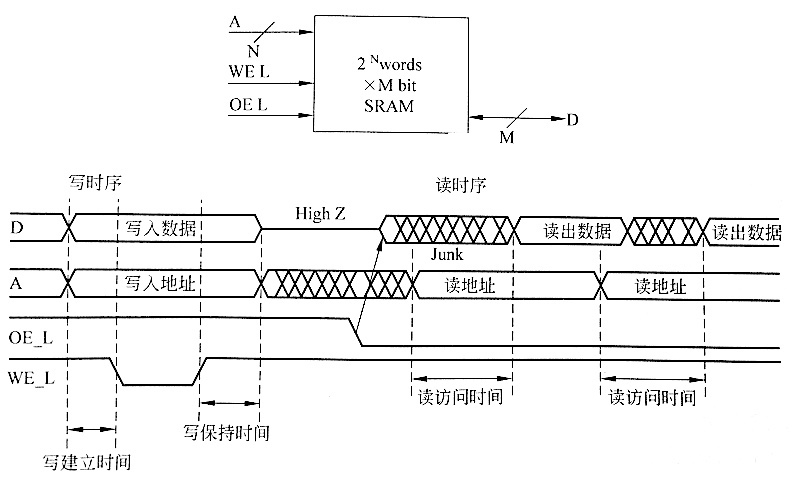
\includegraphics[width=\linewidth]{Figures/SRAM.jpg}
  \caption{SRAM访问时序}
\end{figure}

对于写操作,事先对地址线、数据线赋好值,然后将WE使能拉低,保持一段时间之后拉高,就完成了写入操作。

对于读操作,保持OE使能为低,WE使能为高,对数据线赋高阻,地址线赋为要读取的地址,经过一段延迟时间之后数据线稳定,可以读出数据。

实验使用的SRAM芯片的建立时间、保持时间、读数据延迟等主要参数都在10ns左右。我们在实验中,每个流水段由上升沿驱动,在上升沿根据当前指令的读写情况进行对数据线、地址线赋好值,在下降沿给使能信号赋值,读操作拉低OE使能,写操作拉低WE使能,然后在下一个上升沿到来时拉高。由于信号不能同时被时钟上升沿、下降沿驱动,实际上是根据状态直接把时钟信号赋给使能信号,而不再使用时序逻辑。读操作时,后面一个阶段在下一时钟周期直接从RAM1或RAM2的数据线中获取读出的值。

指令寄存器RAM2在IF阶段访问,在CPU运行时一般只需要进行读操作。但是有两个特殊情况,一是监控程序的A命令,用户输入程序需要写入指令寄存器RAM2,二是boot阶段,系统从Flash中读取数据,写入RAM2中。IF阶段默认执行读操作,对于第一种情况,执行的指令还是SW指令,在MEM阶段发现需要写入RAM2控制的地址空间,则给IF段发出一个写信号,IF阶段接收到信号后改为进行写操作,当前周期输出NOP,即插入一个气泡,所有阶段暂停一个周期,下一个周期再重新执行原来要执行的指令。对于第二种情况,在boot阶段Flash控制器给IF段一个写信号,IF同样改为写操作,输出NOP,暂停一个周期。

一个小技巧用于解决监控程序的U命令,即反汇编,需要在MEM阶段读指令寄存器RAM2。正常情况下IF阶段访问指令寄存器RAM2,MEM阶段只能访问数据寄存器RAM1,无法读取指令。为了解决这个问题,我们发现写指令寄存器的操作都是执行到了MEM阶段,然后返回IF阶段暂停当前周期,写入指令。这时MEM阶段可以同时把写入RAM2的数据也写入一份到RAM1,这一操作在电路中完全并行,互相毫不影响。这样在U命令读取指令时,就无需真的再访问RAM2读指令,直接从RAM1中读取我们备份的指令就可以了。

\subsection{Flash存储器}
我们将监控程序写入Flash存储器中,由于Flash断电数据不丢失,以避免每次写入监控程序的麻烦。

每次开机之后进行boot阶段,将Flash存储器中的数据依次读出,写入RAM2的对应位置。由于此时RAM2执行写操作,流水线暂停直到写入完毕。

Flash的写入使用Flash\& RAM软件写入即可,读操作需要进行一些时序的操作。具体为:首先写入操作码0xFF,地址任意,即设置写使能WE为0,将数据线置为00FF,下一个周期将WE置为1,数据已经写入,Flash进入读模式。读操作需要置读使能OE为0,地址线赋为要读取的地址,数据线赋为高阻,经过一段时间延迟可以读出数据。由于Flash的延迟相对比较大,我们使用的是25MHz时钟,一个时钟周期内Flash读出数据还不稳定,因此两个周期读一个数据。另外要注意的是,Flash的编址方式和RAM1、RAM2不同,使用按字节编址。


%----------------------------------------------------------------------------------------
%	SECTION 4
%----------------------------------------------------------------------------------------

\section{中断处理}

我们实现了四种类型的中断,其中包括两种硬件中断(ESC中断:返回到中断PC;Control C中断:返回到监控程序),软件中断,时钟中断。对这四种中断分别介绍如下。

\subsection{ESC硬件中断}

ESC硬件中断是在用户程序运行时,键盘摁下ESC键产生的中断,在监控程序运行时无效。ESC中断发生时,调用中断处理程序输出中断号,并返回到发生中断的指令继续执行。

这部分硬件中断会复用监控程序的delint中断处理代码,在中断处理程序中需要用到中断时的PC以及中断号,所以需要在发生中断时通过硬件来保存PC与中断号,并跳到中断处理程序。在IF$\_$ID的段间锁存器中加入状态机,来处理ESC中断。状态机见Figure 3.3.

\begin{figure}[H]
  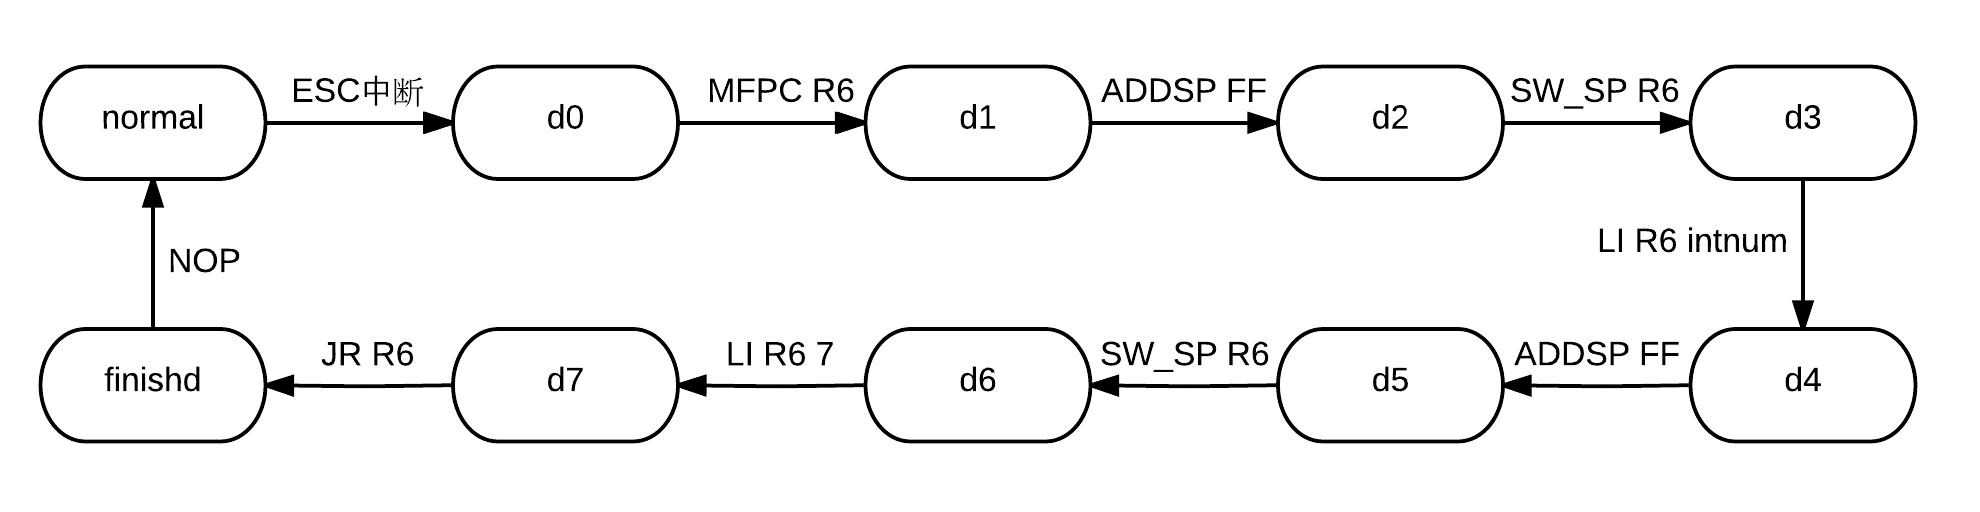
\includegraphics[width=\linewidth]{Figures/escint.png}
  \caption{ESC硬件中断状态机.}
\end{figure}

其中箭头上的指令为每个状态机下输出的指令,用来向栈中存储PC值和中断号。保存完毕后,跳到中断处理程序执行,同时状态回到normal。

\subsection{Control C硬件中断}

ESC硬件中断的不足在于对于死循环的用户程序,中断发生后无法跳出死循环,而是继续回到中断发生的位置执行。我们希望仿照真正计算机上的Control C功能,可以实现跳出用户程序的功能。

Control C中断的处理与ESC硬件中断类似,但是不需要再次返回中断时的PC,而是直接跳到监控程序的BEGIN部分即可。所以处理过程比ESC更加简单,只需要在中断发生后将中断号入栈即可,不需要保存PC值。同时需要在监控程序中加入Control C中断的处理。状态机见Figure 3.4.

\begin{figure}[H]
  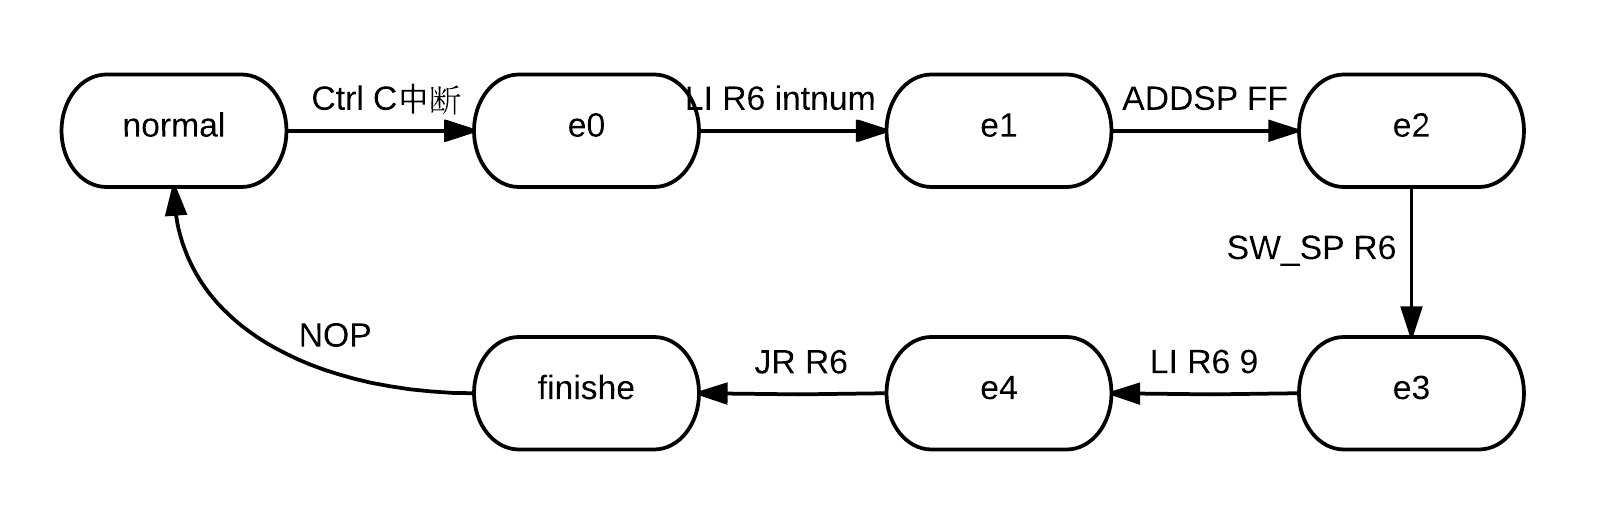
\includegraphics[width=\linewidth]{Figures/ctrl_c.png}
  \caption{Control C硬件中断状态机.}
\end{figure}

\subsection{软件中断}

软件中断的原理与ESC硬件中断一样,通过在控制器译码时产生软件中断的信号,传到IF$\_$ID段间锁存器,同时将软件中断号同时传回,按照ESC的状态机处理软件中断。

\subsection{时钟中断}

时钟中断指计时时钟到一定的时间后,产生中断信号。我们做时钟中断的原因是为了之后的多道程序,多道程序需要分时执行两套监控程序,故需要有分时机制。多道程序的细节在后面讨论,这里仅讨论一下时钟中断的处理。

时钟中断的处理过程与ESC硬件中断基本一致,但是需要注意的一个地方是ESC硬件中断只会发生在用户程序中,这时我们就可以随意使用R6、R7的值(因为用户程序不允许使用)。但是时钟中断可以发生在任何地方,在执行监控程序时也会有时钟中断,所以要首先保存R6的值,才可以执行后续的保存现场的指令。状态机见Figure 3.5.

\begin{figure}[H]
  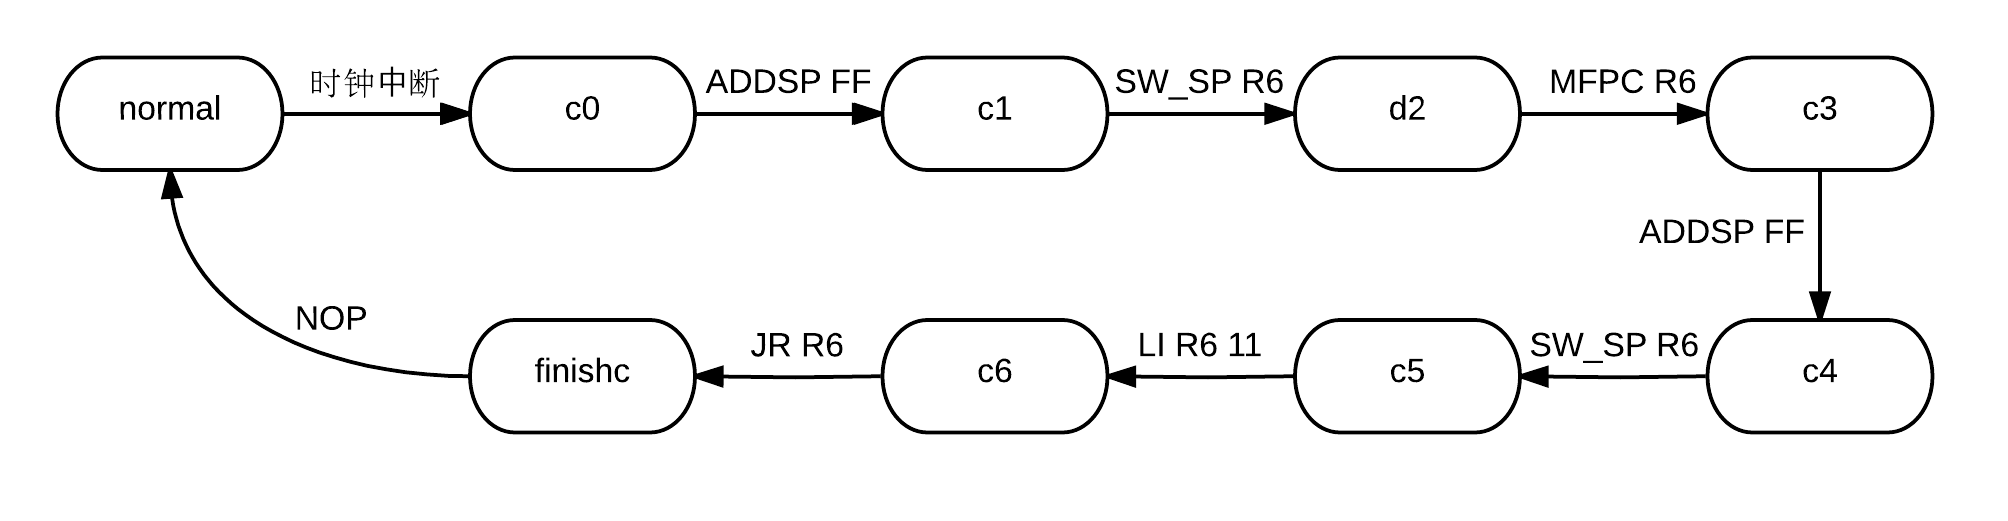
\includegraphics[width=\linewidth]{Figures/clock.png}
  \caption{时钟中断状态机.}
\end{figure}



%----------------------------------------------------------------------------------------
%	SECTION 5
%----------------------------------------------------------------------------------------

\section{I/O}

我们实现了基础版本和扩展键盘VGA的两种CPU。对于基础版本,通过串口与主机term通信。对于键盘VGA版本的CPU,输入输出变成了键盘和VGA,实现了一个完全独立的VGA版的term软件。此版本的term软件实现了主机的term的全部功能,包括A指令输入汇编指令、G指令执行、U指令查看反汇编的指令、D指令查看内存、R指令查看寄存器的值。

\subsection{串口输入输出}

THINPAD教学计算机的FPGA芯片通过基本总线连接了存储器芯片RAM1以及被配置为UART的扩展芯片CPLD。UART连接RS-232接口,作为串口与其他设备连接。串口通信功能已经在CPLD中实现,所以我们仅需要根据串口的访问时序读写总线即可。

我们通过阅读监控程序,了解到读写串口是通过LW/SW指令访问BF00及BF01地址实现的(访问BF01以判断串口是否可读或可写)。所以我们在MEM阶段加入了判断,根据读写地址是否为BF00及BF01判断是否为串口访问。对于BF00,我们只需在数据总线上赋予或读取相应的值,然后将串口通信的信号wrn或rdn拉低即可。对于BF01,我们只需在数据总线的第0位赋予tsre$\&$tbre,第一位赋予data$\_$ready,从而判断串口状态。

和普通的串口芯片8251不同,教学机上的UART没有设计缓冲,也不具备可编程的性质,所以CPLD实现的串口功能有所欠缺。在基础功能的实现中,串口的访问没有遇到很大的问题,但是在后面的多道程序中,如果设置时钟中断的切换时间较长,那么串口则不能保存数据,所以如果在读写过程中发生时钟中断,很容易造成丢失数据,使得term无法正常工作。后面一节会详细讨论多道程序的实现。

\subsection{键盘输入}

键盘主要状态机有13个状态,分别为delay, start, d0, d1, d2, d3, d4, d5, d6, d7, parity, stop, finish,称为R状态机整个状态机使用键盘时钟驱动,根据实验书上内容,当数据线上有数据读入时,首先会将数据线拉低,然后时钟每跳变一次,数据线上将会传入下一个值,将数据按位依次存入到code中,由于键盘在串行传入数据时候可能存在数据出错,因此在接受完数据后需要判断数据校验位,如果数据存在问题,则将数据丢弃并回到起始状态,重新串行读入数据。
	根据这个状态机,我们可以在状态为stop时接受到一个完整数据,在下一部分将对接受到的数据进行处理,使用一个数据通道和一个使能通道传入给键盘状态机模块。具体的状态机见Figure 3.6.
\begin{figure}[H]
  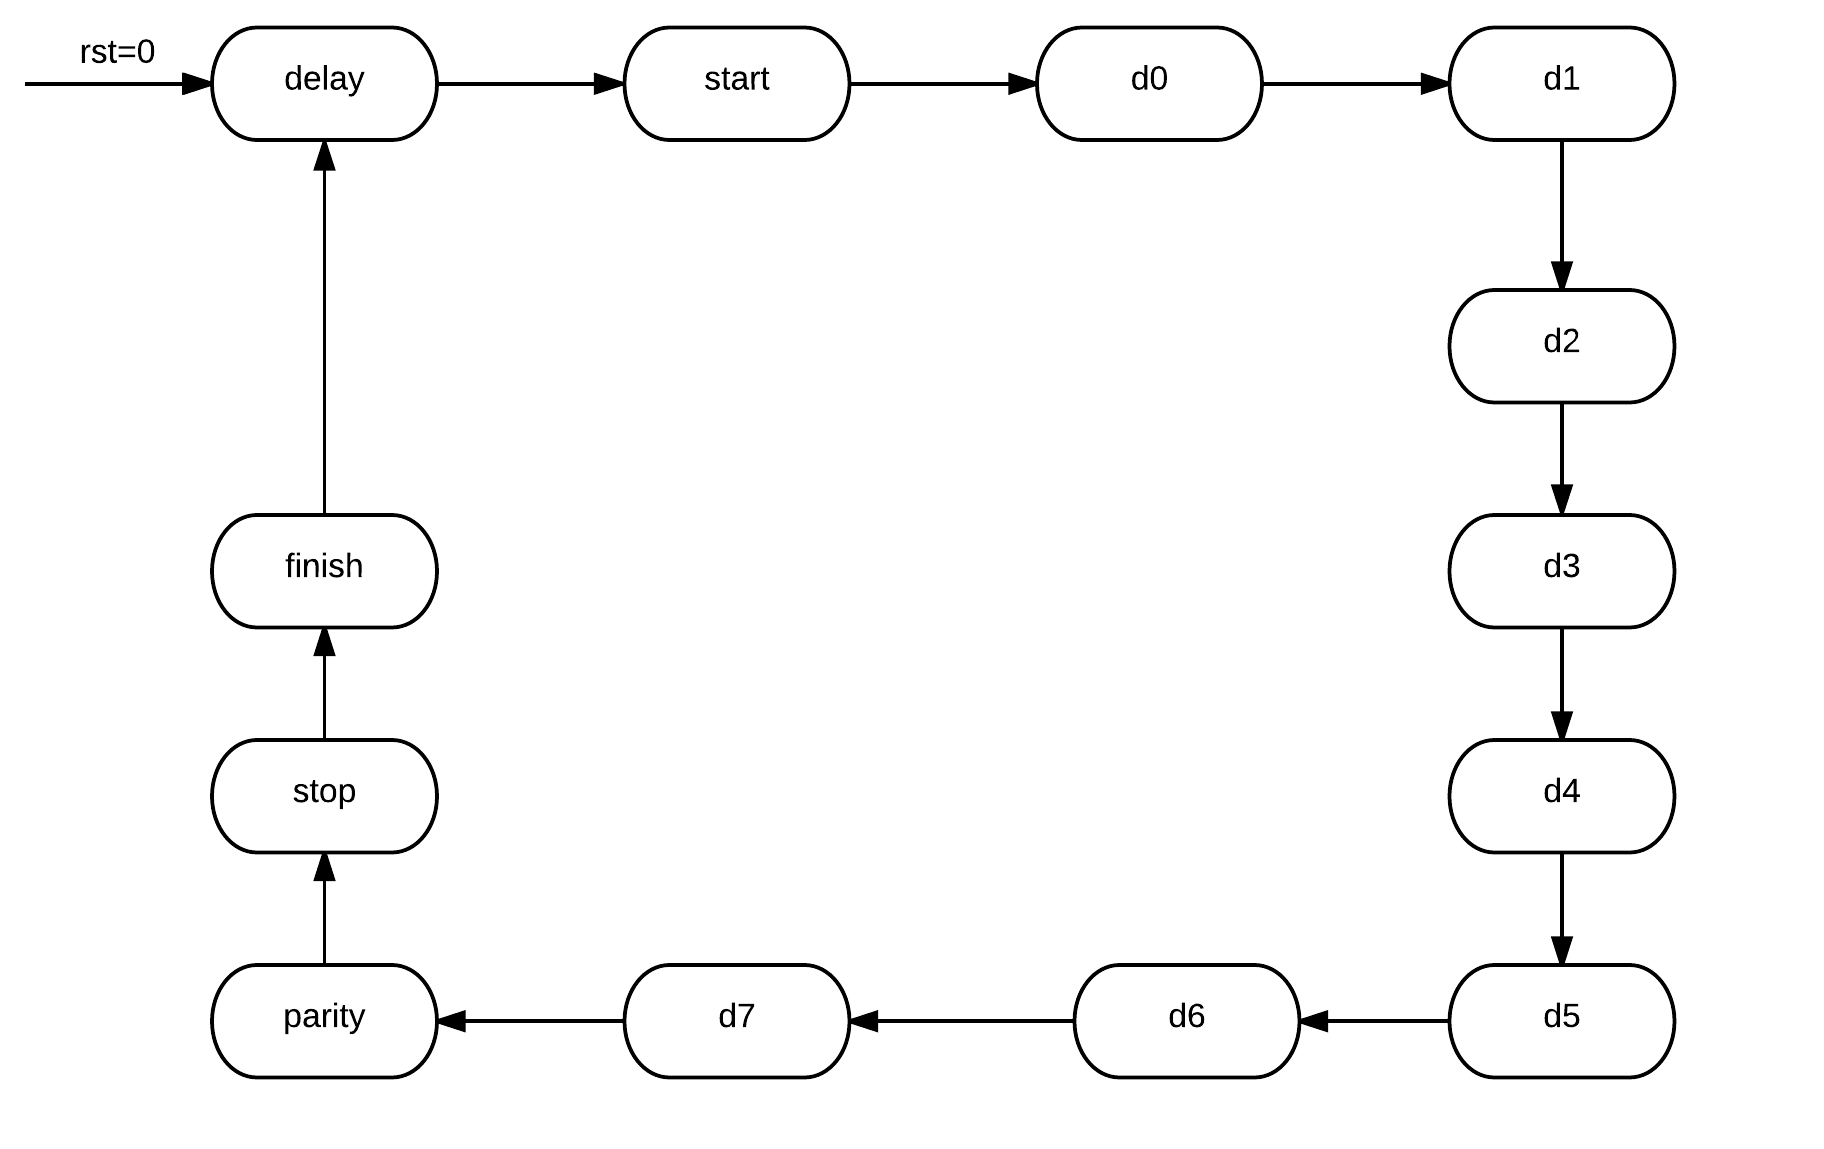
\includegraphics[width=\linewidth]{Figures/keyboard_main.png}
  \caption{键盘}
\end{figure}

对于键盘输入的处理,有两个状态move\_state和wait\_state,称为S状态机在上一部分中,已经能够获得串行读入的数据,键盘数据在正常按下后,会发送一个编码,在放开键盘后,会依次发送一个断码F0和该键的编码,需要注意的是,如果按下一个键不放,在经过一个比较短的时间后,键盘将会连续地发
送同样的编码。

根据这样的特点,设计了两个状态的状态机,根据读入的编码来选择状态转变,如果读入的编码为F0,会进入wait\_state而在进入wait\_state时需要判断读入的编码,如果不是先前读入的键的编码,则回到move\_state。键盘模块传入给键盘上层模块的数据线使用当前存入的按下的键,即当按下一个键不放时,数据线上并行传入当前按下的键,放开键后,数据线全部赋为低电位。在本键盘中,为了能够尽量真实地模拟键盘,当在按下A键时再按下B键时,数据线上将赋值为B键。

\begin{figure}[H]
  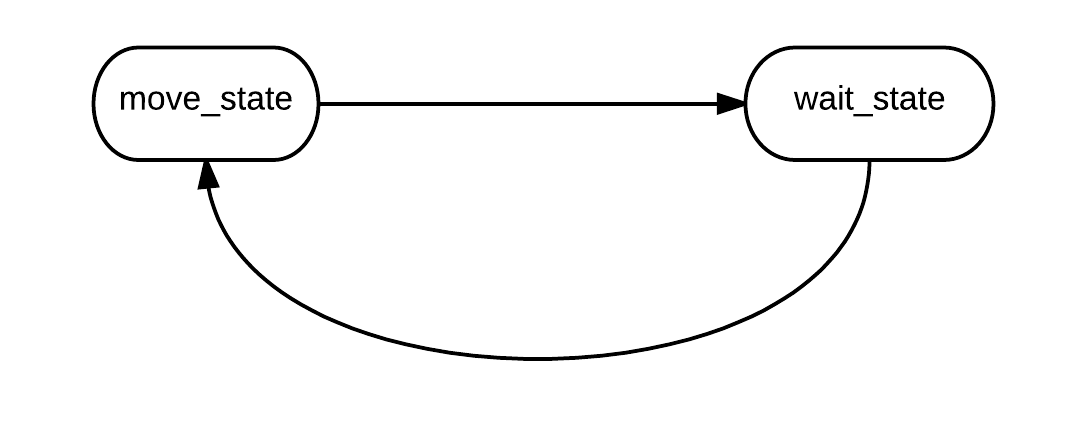
\includegraphics[width=\linewidth]{Figures/keyboard.png}
  \caption{键盘输入}
\end{figure}

键盘上层模块将根据使能位对数据进行读取处理。在前一章状态机中,在start状态机内,会将使能位拉低,而在stop状态机内,根据S状态机状态和当前键盘读入的数据判断是否将使能位拉高,在读入到一个普通编码(非断码,非shift,ctrl)后使能位被拉高。这样做的好处在于可以真实地模拟键盘在长按一个键的情况,在这样的情况下,键盘上层可以根据使能位不断读入一串字符。

键盘模块中还会发出三种特殊信号。信号为是否按下shfit,是否按下ctrl,是否按下中断键(ESC键),shift键和ctrl键的处理方式相同,在按下shift/ctrl键时,对应的数据位为高,放开shift/ctrl键后,对应的数据位为低,上层模块根据shift/ctrl键来判断是否按下shift或ctrl键。中断按键处理方式类似于普通按键,在此不再赘述。

对于我们实现的term程序的A、G、U、D、R五条指令,通过判断缓冲区中的字符来进行发送。为了尽量不改变监控程序以及CPU的代码,我们让键盘仿照串口,通过BF00和BF01端口输入,同时增加使能信号rdn、data\_ready来进行数据发送。同时将数据放到数据总线上,完成键盘输入功能。

\subsection{汇编码转为机器码}

我们在实现键盘VGA时,为了尽量模拟主机term程序的功能,加入了A指令输入汇编码的功能。由于监控程序的输入指令为机器码表示,所以我们需要在键盘给CPU发送数据之前将用户输入的汇编码转为机器码。通过compiler模块实现。

compiler模块的输入为指令缓冲区,用断码表示汇编码的每个字符,输出为16位的机器码指令。我们加入了一部分的代码检错功能,对于不合法的汇编指令,翻译成的机器码全为1,然后指示用户重新输入此条指令。基本做到了与term程序一样的汇编码输入功能。

\subsection{VGA输出}

我们实现了使用VGA接口输出,在显示屏上显示计算机运行的信息。

仿照终端程序Term,我们输出的界面是一个命令行的界面,即一个字符的阵列。我们VGA的输出使用分辨率为$640\times 480$像素的显示模式,故规定屏幕上显示30行、80列字符,每个字符的显示大小为$16\times 8$像素。

为了实现命令行的界面,我们使用实验FPGA芯片提供的片内BlockRam作为显存。具体地,我们例化了两块显存,一块双端口Ram,用于存取字符阵列信息,另一块是单端口Rom,用于存取所有可见ASCII码的字体图片。Ram的地址线12位(5位表示行、7位表示列)、数据线16位,存放字符。Rom的地址线14位(7位表示ASCII、4位表示行、3位表示列)。

有了显存的帮助,尤其是有双端口Ram的情况下,我们只需要在每次有输入数据的时候,将数据写入Ram,然后VGA在行、场信号扫描时,根据坐标从Ram中读出字符信息,再从Rom中读出该字符在当前位置的颜色,用VGA输出出来。这些过程都可以独立同时进行,而不会造成访存的冲突。

在硬件程序中还需要做一些命令行界面的控制,包括存储每一行有多少个字符,处理删除、回车、换行、换页等情况,以及显示光标。具体地,在硬件语言中需要维护一个数组记录当前每行的长度(即已有字符的个数,左对齐显示),以及维护当前在哪一行。这样有输入数据时,除了要往Ram里写入数据,还要增加当前行的长度。如果是删除操作,就减少当前行的长度。在显示时,不完全按照Ram中存放的数据,超过当前行长度后面的字符均不显示,所以删除操作也不需要抹去Ram中的存储。如果是换行操作,则需要更新当前行,即进入下一行。这里会有一个换页的情况,如果写到最后一行(第30行)换行,那么第一行就没有用了,返回到第一行继续写。为了显示的一致性,需要记录一个offset,即目前存储中实际的第一行是哪一行。光标的显示,在当前行行末的一个字符交替显示黑白即可实现。

\subsection{屏幕保护界面}

我们将上一学期《数字逻辑设计》的课程项目经过简化后加入我们此次的计算机实验,作为屏幕保护界面呈现出来。具体就是在一段时间没有用户键盘的输入、CPU也没有输出的情况下,显示屏进入另外一套VGA的控制,显示屏幕保护界面。

我们的屏幕保护界面内容是一系列小球围绕中央转动的动画。实现上,根据时间变化计算小球的坐标,然后绘制圆、直线,通过VGA显示。由于$640\times 480$像素的分辨率比较低,我们在实现上还应用了计算机图形学的知识,对画圆、画直线算法进行了消锯齿处理。

\subsection{机器码转为汇编码}

同样,为了模拟term程序的U指令反汇编的功能,我们加入了机器码转为汇编码输出的模块。由于硬件显示为时序逻辑,且延迟较难处理,我们把反汇编功能放到软件上实现。通过改写监控程序,将16位的机器码转为汇编码,然后逐字发送到VGA显示。


%----------------------------------------------------------------------------------------
%	SECTION 6
%----------------------------------------------------------------------------------------

\section{多道程序}

我们实现了扩展功能中的多道程序。在同一台教学计算机上可以连接两个终端,同时运行各自的监控程序,并可以互不干扰的运行不相同的用户程序。

考虑到我们已经较好地实现了键盘VGA模拟的term程序,这样我们就可以将键盘VGA的term程序看做第二个终端。这样,教学计算机同时与电脑端的term通信,也与键盘VGA的term通信。多道程序的实现原理为分时机制,我们之前介绍过的时钟中断在这里派上用场。通过时钟中断,CPU在两套监控程序中切换,这样就可以同时运行两套监控程序。

我们将地址单元进一步划分。

\begin{table}[H]
\begin{center}
\renewcommand{\arraystretch}{1.3}
\small
\caption{Memory Allocate}
\label{tab:treatments}
\begin{tabular}{|p{3cm}<{\centering}|p{3.5cm}<{\centering}|p{3.5cm}<{\centering}|}
\hline
 & 电脑端term & 键盘VGA \\
\hline
监控程序 & 0x2000-0x3FFF & 0x0000-0x1FFF \\
\hline
用户寄存器 & 0xBF10-0xBF15 & 0xBF16-0xBF1B \\
\hline
栈顶指针 & 0xBF50 & 0xBF60 \\
\hline
保存现场缓存区 & 0xBF20-0xBF2F & 0xBF30-0xBF3F \\
\hline
\end{tabular}
\end{center}
\end{table}

在实现多道程序时,我们遇到了很多问题,除了时钟中断外,在设计上也遇到了很多挑战,我们详细说明如下。

由于时钟中断会发生在监控程序中,所以我们在处理中断使用寄存器之前要首先将寄存器的值保存。所以在处理时钟中断时,我们不能使用没有保存过的寄存器。同时,在跳转到另一套监控程序之前,也需要将各个寄存器的值恢复,才能跳转。除了保存寄存器之外,还要保存当前的PC、栈顶指针SP等。

由于两套监控程序的栈顶指针寄存器地址不一样,所以中断发生时要保存SP,再恢复另一套监控程序的SP。但是在指令集中我们没有发现读取当前SP到某个寄存器或地址的指令。这样就不能保存栈顶指针的值。所以我们需要扩展指令获取当前SP的值,然后进行保存。考虑到新创建指令Assembler不能编译的问题,我们复用SLTUI指令,并将其解析为将SP值保存到寄存器中。

在恢复现场时遇到的另一个问题为在中断处理的最后需要跳到另一套监控程序的PC值,这时候我们需要通过JR指令进行跳转,但是需要一个寄存器保存跳转的PC。问题是所有寄存器需要保存之前的值,没有多余的寄存器来保存跳转的地址。为了解决这个问题,我们采用了一种简单的办法,就是打开跳转的延迟槽。首先我们将R6的值放在栈中,然后让R6保存跳转的PC,通过JR R6实现跳转,然后在跳转的延迟槽中将栈中的R6值恢复。


\textbf{\textit{Example5}}: \quad SW\_SP R6 0xFF; \quad LI R6 PC; \quad JR R6; \quad LW\_SP R6 0xFF





